\chapter{Modelos Te\'{o}ricos}
La din\'{a}mica de una biomol\'{e}cula se determina por las ecuaciones de movimiento para cada uno de los \'{a}tomos que la constituyen. Usualmente en una biomol\'{e}cula el n\'{u}mero de mon\'{o}meros es mayor a 20, que al multiplicarlo por el n\'{u}mero de \'{a}tomos en cada mon\'{o}mero incrementa considerablemente el n\'{u}mero de ecuaciones de movimiento a resolver, de ah\'{i} que sea necesario realizar \textit{din\'{a}mica molecular} (Molecular Dynamics por sus siglas en ingl\'{e}s MD) la cual estudia mediante simulaciones computacionales el movimiento de los \'{a}tomos, de acuerdo a las interacciones que presenten.\\

Las ecuaciones de movimiento se pueden conocer a partir de los formalismos lagrangiano o hamiltoniano, en los cuales es necesario conocer los potenciales con los que interact\'{u}an los \'{a}tomos. Las soluciones a las ecuaciones de movimiento se encuentran mediante los m\'{e}todos de la din\'{a}mica molecular o los an\'{a}lisis de modos normales (Normal Mode Analysis por sus siglas en ingl\'{e}s NMA).

Los diversos modelos de potencial pueden ser tomados según la naturaleza del pol\'{i}mero a analizar, ver \cite{Amb1}. Sin embargo, al escoger el potencial  para hacer un an\'{a}lisis \textit{in silico} de la din\'{a}mica de una biomol\'{e}cula, debe tenerse en cuenta el costo computacional requerido, esto es, el tiempo de simulaci\'{o}n de la mol\'{e}cula y la exactitud en el movimiento de cada uno de los constituyentes de la mol\'{e}cula.

De acuerdo a los par\'{a}metros de costo y tiempo, las simulaciones de biomol\'{e}culas se pueden hacer analizando los \textit{movimientos locales} y los \textit{movimientos globales}.

\section{Movimientos Locales}
Hace referencia a las simulaciones en las que se incluyen todos los \'{a}tomos junto con las interacciones presentes, es decir, en las que se analizan los \textit{cambios locales}. Estas se pueden simular a un orden de magnitud de los nanosegundos en una m\'{a}quina usual, al respecto ver \cite{glo}.

Como caso particular se pueden tomar los potenciales usados en \cite{Amb1} y en \cite{web:Amb2}, que siguen el modelo de Amber. El modelo de Amber tiene en cuenta las contribuciones debidas a:
 \begin{itemize}
\item Interacciones intermoleculares: Son las producidas por los enlaces covalentes entre grupos de \'{a}tomos, las de valencia y las torsiones.
\item Interacciones entre pares: Lennard Jones, electrost\'{a}tico.
\end{itemize}

\section{Movimientos Globales}

Son aqu\'{e}llas simulaciones en las que se desean conocer los \textit{cambios globales} o, el aspecto general que excibe el movimiento de una biomol\'{e}cula haciendo simplificaciones ya sea en los potenciales presentes en la biomol\'{e}cula como en el el n\'{u}mero de \'{a}tomos interconectados. Este tipo de simulaciones pueden ser realizadas a un orden de magnitud de los microsegundos, lo cual facilita su uso en computadores personales, ver \cite{glo}.

Un conjunto de modelos que permite calcular los movimientos globales de una mol\'{e}cula son los \textit{Modelos de Redes El\'{a}sticas} (Elastic Network Models o ENM por sus siglas en ingl\'{e}s).

\subsection{Modelos de Redes El\'{a}sticas (ENM)}
Los ENM, como la palabra \textit{el\'{a}stico} lo indica, se basan en una simplificaci\'{o}n de la energ\'{i}a potencial a una energ\'{i}a potencial el\'{a}stica, es decir de tipo Hooke. Un requisito para que sea posible hacer dicha simplificaci\'{o}n, es el hecho de que sea posible \textit{minimizar} la energ\'{i}a potencial.

Al simplificar el potencial, la biomol\'{e}cula original se convierte en una red cuyos nodos est\'{a}n sometidos al potencial el\'{a}stico, ver figura \ref{fig:pan}; los nodos se consideran como bloques constituyentes de la biomol\'{e}cula y no necesariamente, cada uno de los \'{a}tomos de la biomol\'{e}cula. 
\begin{figure}
\centering%
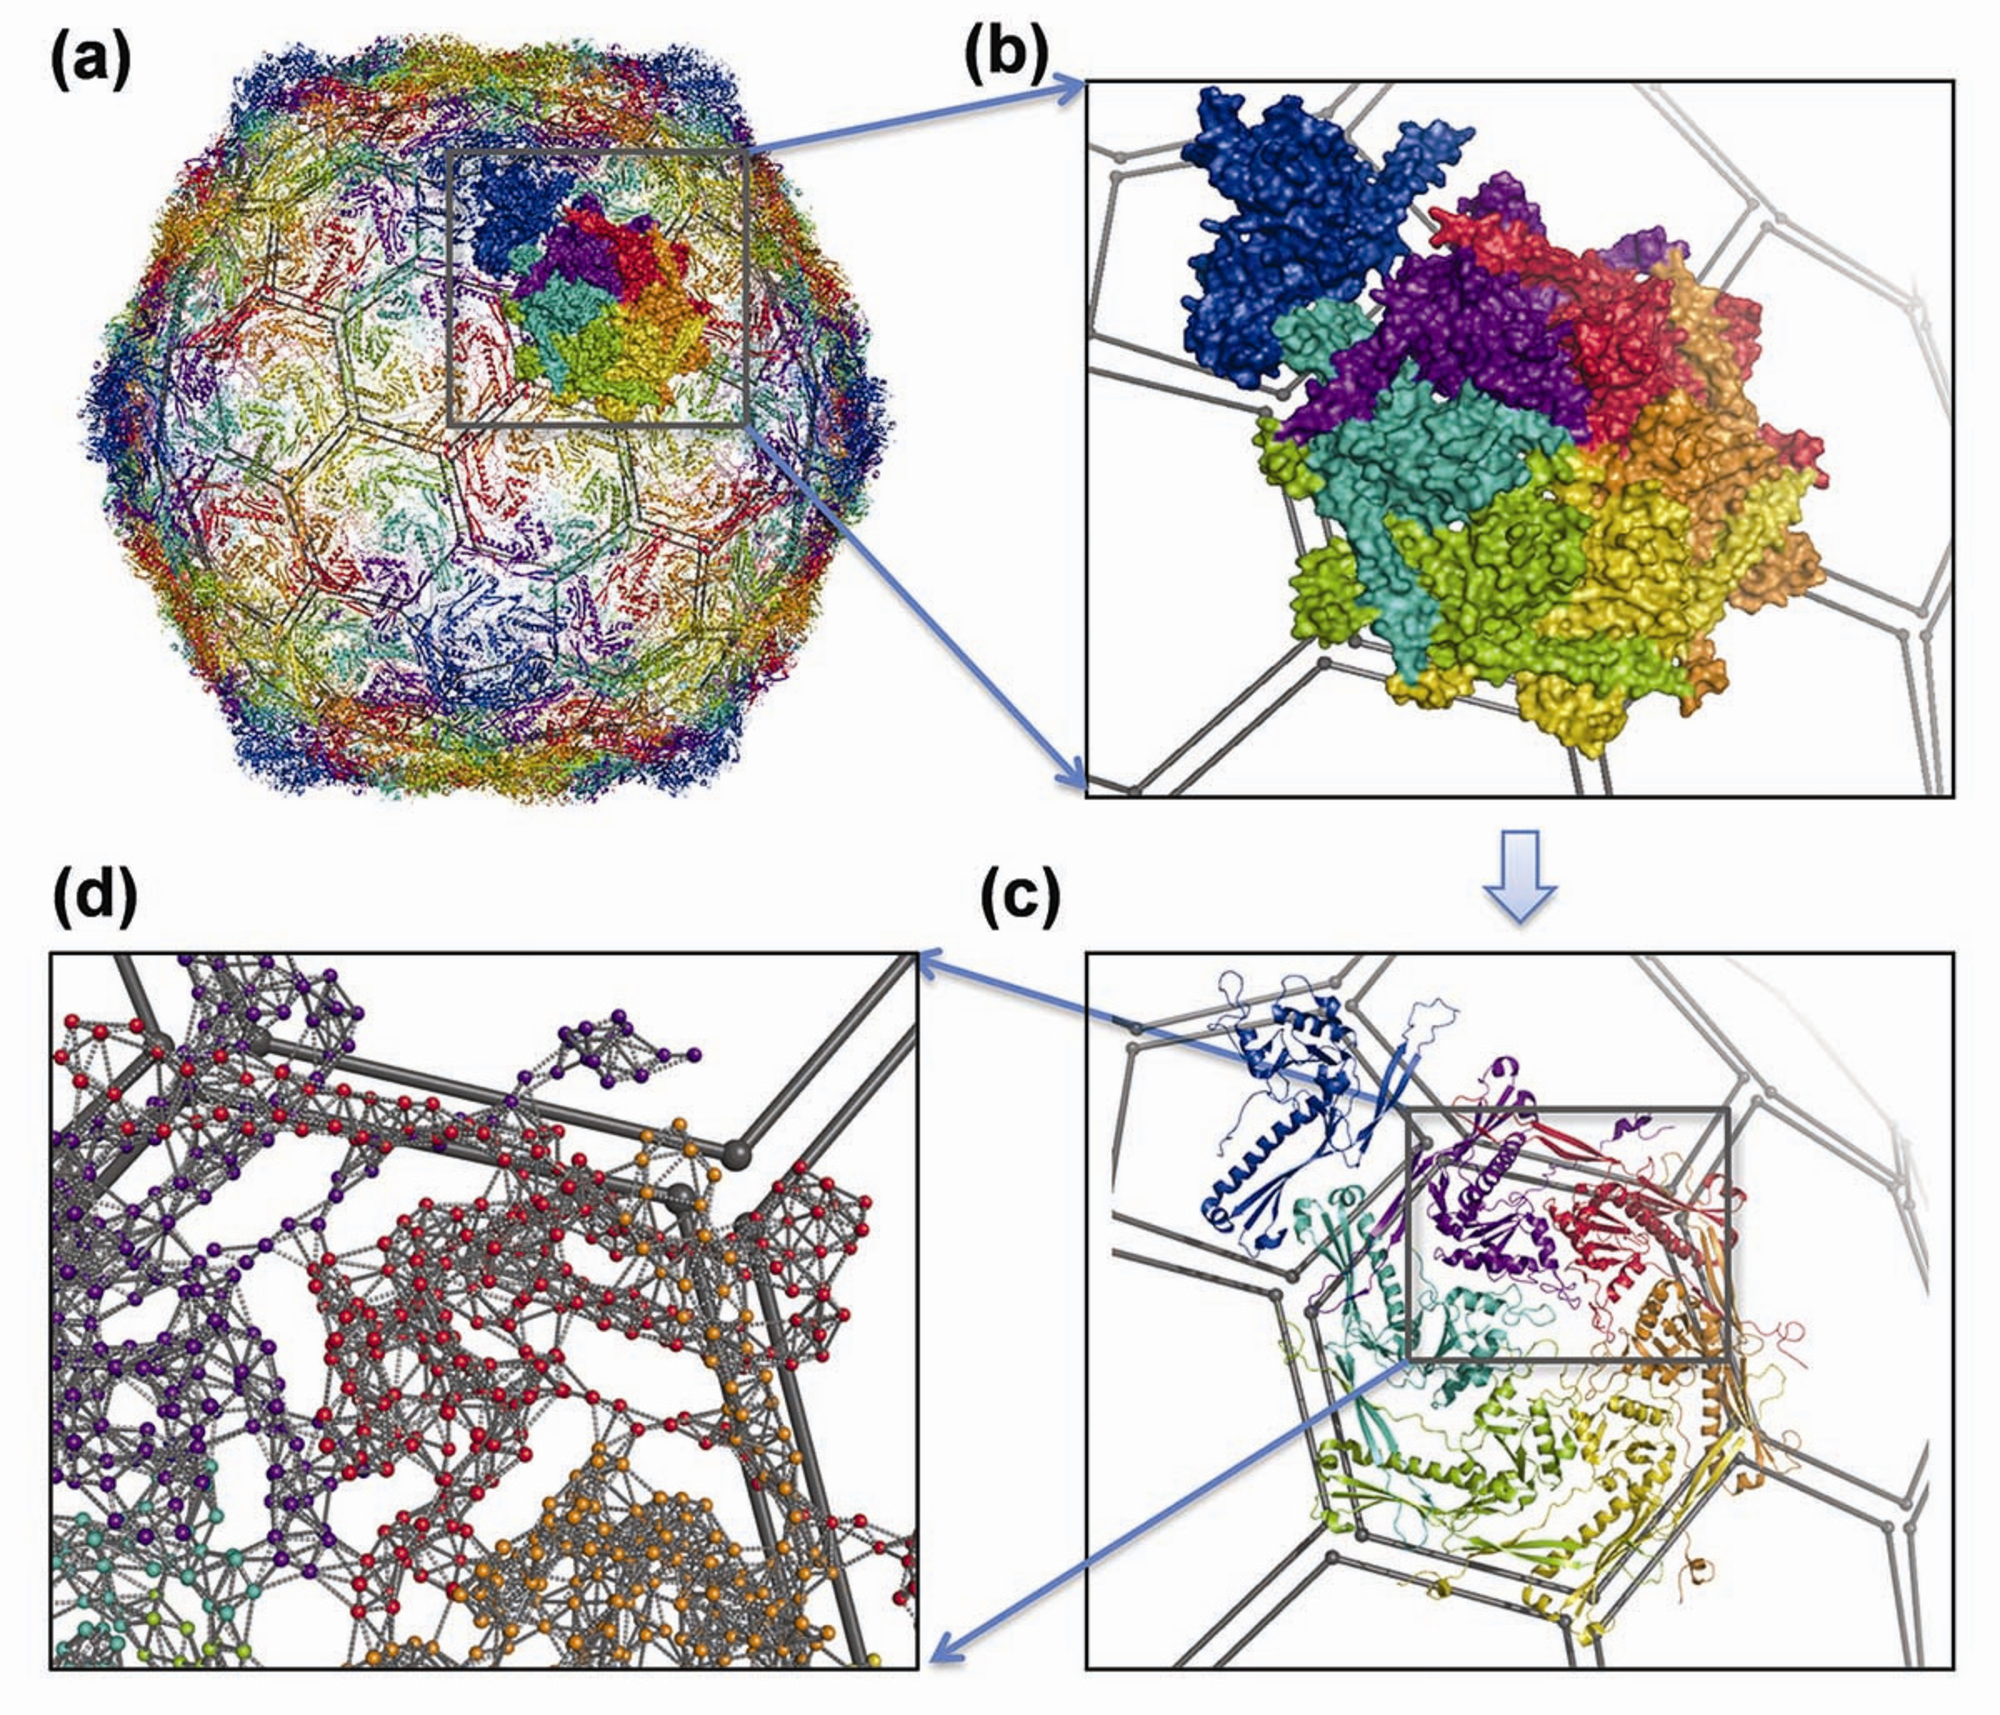
\includegraphics{dibujo.pdf}%
\caption{ (a) Vista exterior de un c\'{a}pside v\'{i}rico HK97 coloreado por cada cadena, todas las prote\'{i}nas son id\'{e}nticas. (b) Vista del arreglo prote\'{i}nico en una cara del c\'{a}pside. (c) Vista de la estructura secundaria de las prote\'{i}nas (d) Esquema de cada prote\'{i}na mostrando cada uno de sus \'{a}tomos, las aristas de cada cara son carbonos $\alpha$ unidos por lados (ligaduras el\'{a}sticas. Tomado de \cite{AG03p,AG04p}.} \label{fig:pan}
\end{figure}
\subsubsection{Descripci\'{o}n Mec\'{a}nica del Modelo}

Consid\'{e}rese un biomol\'{e}cula con $N$ 
Para una funci\'{o}n de energ\'{i}a potencial 

\subsubsection{o}


Las subdivisiones, las vi\~{n}etas y sus textos acompa\~{n}antes deben presentarse sin sangr\'{\i}a y justificados.\\

\begin{itemize}
\item En caso que sea necesario utilizar vi\~{n}etas, use este formato (vi\~{n}etas cuadradas).
\end{itemize}
